\documentclass{report}
% Change "article" to "report" to get rid of page number on title page
\usepackage{amsmath,amsfonts,amsthm,amssymb}
\usepackage{setspace}
\usepackage{Tabbing}
\usepackage{fancyhdr}
\usepackage{lastpage}
\usepackage{extramarks}
\usepackage{chngpage}
\usepackage{soul,color}
\usepackage{listings}
\usepackage{enumerate}
\usepackage{graphicx,float,wrapfig}
\usepackage{pifont}
\usepackage{graphicx}
\usepackage[english]{babel}
\usepackage{tikz}
\usepackage{algorithm}
\usepackage{algpseudocode}
\usepackage{cite}
% In case you need to adjust margins:
\topmargin=-0.45in      %
\evensidemargin=0in     %
\oddsidemargin=0in      %
\textwidth=6.5in        %
\textheight=9.0in       %
\headsep=0.25in         %

\title{Project - Comp 652 - Machine Learning}

% Homework Specific Information
\newcommand{\hmwkTitle}{Project}                     % Adjust this
\newcommand{\hmwkDueDate}{Thursday, April 23 2015}                           % Adjust this
\newcommand{\hmwkClass}{COMP 652}


\newcommand{\hmwkClassInstructor}{Dr. Doina Precup}
\newcommand{\hmwkAuthorName}{Geoffrey Stanley}
\newcommand{\hmwkAuthorNumber}{260645907}
\newcommand{\Pp}{\mathbb{P}}
\newcommand{\Ev}{\mathbb{E}}
\newcommand{\cov}{\text{Cov}}
\newcommand{\Z}{\mathbb{Z}}
\newcommand{\R}{\mathbb{R}}
\newcommand{\dd}{\, \mathrm{d}}

% Setup the header and footer
\pagestyle{fancy}                                                       %
\lhead{\hmwkAuthorName}                              %
\chead{}
\rhead{\hmwkClass: \hmwkTitle}                                          %

\lfoot{}
\cfoot{}                                                                %
\rfoot{Page\ \thepage\ of\ \pageref{LastPage}}                          %
\renewcommand\headrulewidth{0.4pt}                                      %
\renewcommand\footrulewidth{0.4pt}                                      %

% This is used to trace down (pin point) problems
% in latexing a document:
%\tracingall
\definecolor{mygreen}{rgb}{0,0.6,0}
\lstset{commentstyle=\color{mygreen}, frame=single,  language=R, showspaces=false, showstringspaces=false}

%%%%%%%%%%%%%%%%%%%%%%%%%%%%%%%%%%%%%%%%%%%%%%%%%%%%%%%%%%%%%
% Make title
\title{\vspace{2in}\textmd{\textbf{\hmwkClass:\ \hmwkTitle}}\\
\normalsize\vspace{0.1in}\small{Due\ on\ \hmwkDueDate}\\
\vspace{0.1in}\large{\textit{Presented to \hmwkClassInstructor}}\vspace{3in}}
\date{}
\author{\textbf{\hmwkAuthorName}\\
    \textbf{Student ID: \hmwkAuthorNumber}}
%%%%%%%%%%%%%%%%%%%%%%%%%%%%%%%%%%%%%%%%%%%%%%%%%%%%%%%%%%%%%

\begin{document}
\maketitle
\subsection*{Introduction}
The reliability of modern day energy markets is the responsibility of
independent system operators (ISO) who are tasked with the governance of the energy
network within a pre-definied geographic region. PJM Interconnection is such an
organization. It is responsible for the proper functioning of the electric grid
in Delaware, Illinois, Indiana, Kentucky, Maryland, Michigan, New Jersey,
North Carolina, Ohio, Pennsylvania, Tennessee, Virginia, West Virginia and the
District of Columbia.

It ensures that loads on the system, such as cities, are
serviced by a sufficient amount of generators, such as nuclear, natural gas or
wind power plants at any given hour of the day. It does so by holding hourly
auctions requesting that producers offer the quantity of megawhatts they are capable of
producing and at what cost. Next, based on the demand for a given hour the ISO
will request that the producers bring their generators online, prioritizing the
most inexpensive power first while also ensuring that the grid operates at a
sufficient level of reliability and redundancy.

The first priority of the ISO is the reliability of the system. If it does not
provide a sufficient amount of power to satisfy the loads in the system it
risks causing a brown out or a black out in the entire system. It also must
ensure a certain level of redundancy as if a line or a power plant suddenly
fails the energy grid must continue to operator as a whole. It's second
priority is to provide loads with the most inexpensive power that it can find,
nuclear is cheaper then natural gas, and natural gas cheaper then coal.

As such, the price of power through out the energy grid can be seen as being driven
by three categories of variables: demand, supply and physical. With in the demand
component variables will be ones that influence the amount of power being drawn from
the grid. These will be things such as weather, season, day of the week, hour of
the day, weather it's a holiday or normal work week. Supply will be made up of all
factors influencing how generators are changing their bidding behavior. This will
mostly be driven by fuel costs; uranium, natural gas, coal and the amount of wind.
Physical variables will be the current status of the network; what outages and
constraints there are on the system.

Congestion...

In order to protect generators from unforseen congestion events products called
up to congestion (UTC) contracts were created...

\subsection*{Methodology}
Ignoring potential variables such as fuel costs, weather and outages, as a a first
attempt in trying to evaluate the value of a UTC contract a Markov
Chain Monte Carlo approach will be used. The objective will be to use the
previous distribution of differences between UTC contract prices and the last
known price to estimate the most likely value in the future.

In order to attempt to reduce the effect of variables outside of normal seasonality
aggregates of nodes were selected; Eastern Hub and Western Hub. These hubs are an average
of a few hundred different pricing nodes within their regions.


Price differences between January first 2013 and January first 2015 did not
fluctuate a great deal except for a period in January 2014. The differences in
price from one hour to the next for this two year period can be seen in the
following figure:
\begin{center}
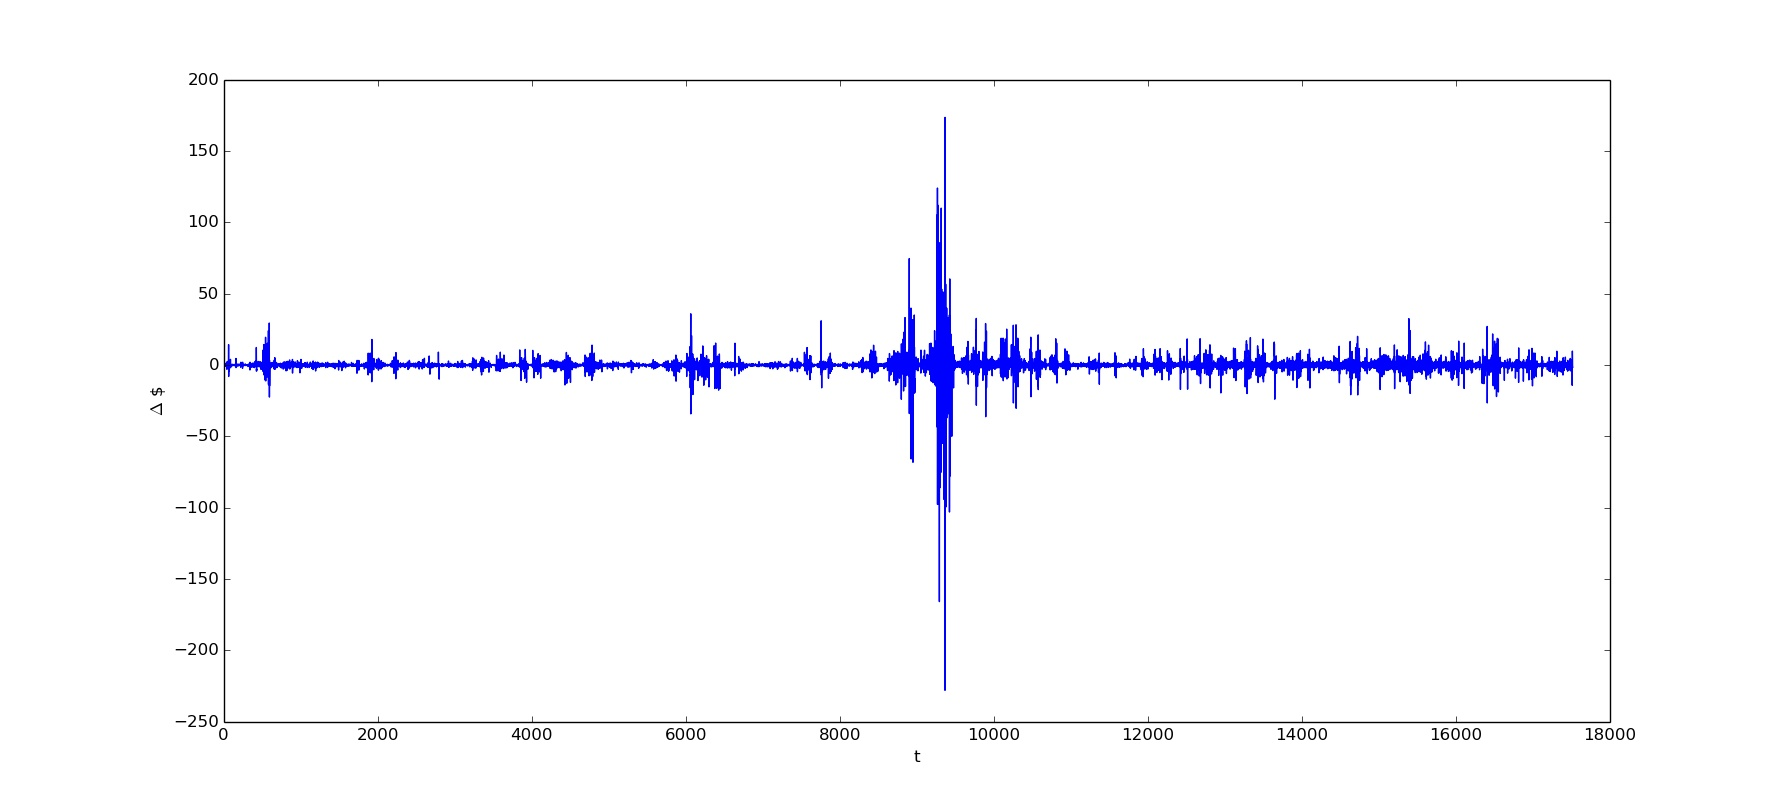
\includegraphics[width=500pt, keepaspectratio=true]{price_differences.jpg}\\
\end{center}
Because of the tendency of price differences to be within a rather tight range
with the exception of a few outliers  10\% of the top and bottom

\begin{center}
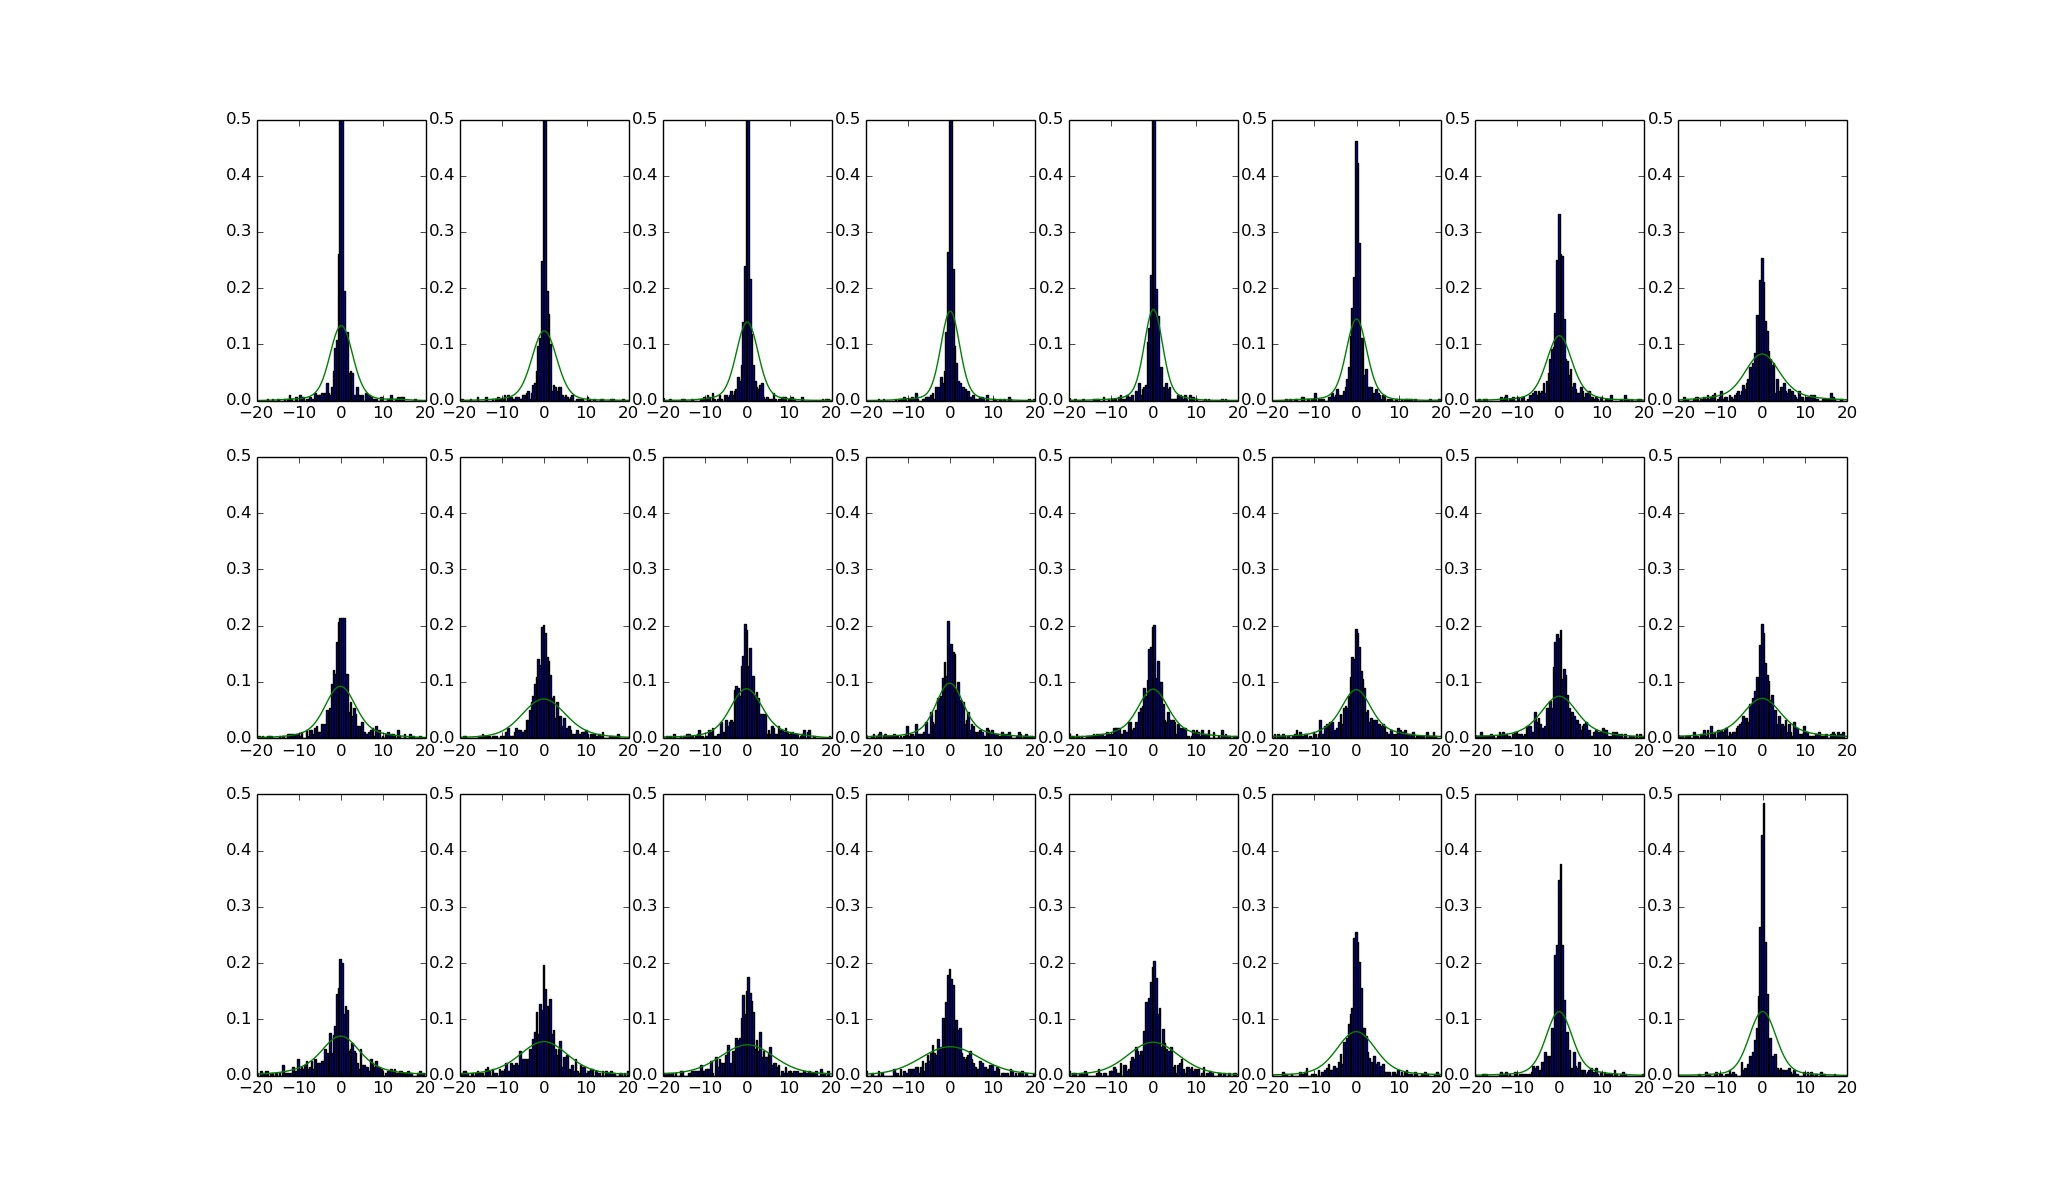
\includegraphics[width=500pt, keepaspectratio=true]{hourly_distributions.jpg}\\
\end{center}


\cite{scipy}
\subsection*{Set-up}
\subsection*{Results}
\subsection*{Conclusions}

\nocite{*}
\bibliography{bibliography}
\bibliographystyle{plain}

\end{document}
